\chapter{Literature Review}
%\label{sec:ob_rel}
\section{Introduction to water quality control}
\subsection{Automated system for water quality control}
%%%%%%%%%%PLC and some real application cases in WTP
%Explain PLC better by \cite{WasteWaterTreatment2018}
%re organize this section
A programmable logic controller (PLC) is an industrial computer system designed for any process requiring a series of devices and equipment to operate cohesively to achieve multiple purposes in manufacturing or treatment processes. The main components of PLC include a central process unit (CPU), input modules, and output modules (I/O). CPU is responsible for processing digital signals from input modules and sending commands through output modules based on the control logic programmed on the PLC. For chemical dosing control in water treatment plants (WTPs), the PLC system receives readings from turbidity and pH sensors and uses pumps to dose aluminum solution automatically \citep{andhareSCADAToolIncrease2014}. The PLC system with the capability of producing real-time output commands in response to the input signals also makes it widely used in wastewater treatment plants (WWTPs). For oxygen concentration control in the aeration tank, the PLC system receives signals from dissolved oxygen (DO) detectors and transmits signals to open or close the electric butterfly valves to alter the DO concentration \citep{zhuApplicationPLCSewage2017}. Although PLC systems are the most used systems across industries for their easy programming and reliable control, PLC system is merely a device that can be programmed to control operative devices with on-off logic (i.e., a logic control with two states). The straightforward implementation of the PLC system compromised its ability to perform complex tasks in a more dynamic water treatment environment. In reality, many WTPs or WWTPs require precise control of the treatment processes. Being aware of the limitations of the PLC systems, a more advanced controller called proportional–integral–derivative (PID) controller for receiving analog signals was developed to obtain more sophisticated controls over the operative devices.

%%%%%%%%%%PID and examples
%PID control is used where greater levels of precision in control are required. It combines three control terms to give a single output to drive the setpoint. 
To react to rapidly-changing environments in wastewater treatment plants, a PID controller generates an output value based on the continuous calculation of an error value e(t), which is the difference between the desired setpoint (SP) and a measured process variable. Then, the controller applies a correction based on proportional, integral, and derivative terms in the control functions. The use of the "P," "I," and "D" allows the system to quickly reach steady-states with feedback control systems (i.e., the system output is returned to the system input, which is included in the decision-making process of PID controller). Generally speaking, a PID controller is a technology (i.e., a specialist algorithm) for controlling a single device with more complex logic, while a PLC system is a physical system consisting of different modules capable of controlling dozens of devices only with two-state logic. In addition, A PID controller can be designed to operate on a PLC device and provide a more specific control strategy to a designated device. In WWTPs, a single-variable feedback analog control loop in PID can be used to control the temperature in the activated sludge treatment by stabilizing the system temperature in a shorter time \citep{badosDesignPIDControl2020}. The feedback control scheme is also applied in DWTPs to adjust the addition of chlorine dosage (i.e., also known as the disinfection process, chlorination, or post-chlorination) to reach the target concentration of free chlorine residual (FRC) \citep{wangCompositeControlPostChlorine2019}. The disinfection process is carried out in a chlorine contact tank, which provides sufficient time for the chlorine to disinfect pollutants. Since the chlorine added by the dosing device requires time to travel from the entry to the exit, the system output can only reflect the changes in water quality in a delayed time of 30 minutes. In the case of chlorination, the time lag makes feedback control difficult \citep{kobylinskiLineControlStrategies2006} as the system is delayed in responding to any sudden surge of the pollutants when it can only receive output at the end of the disinfection process. PID controllers in WWTPs also encounter similar challenges as the increasing complexity of water quality and stricter regulations on the discharged water quality. 

%%%%%%%%%%Transition to how the algorithms in PID can be replace by AI, ML, 
%Introduce to MPC, feedforward control in comparison with PID controller
%The use of mathematical modeling is not ideal, turning to the use of AI modeling
Many control strategies are proposed to address the challenges encountered in the process control system. For instance, feed forward-feedback control, linearized and optimal control, model-predictive control, fuzzy control \citep{demirFeedbackControlChlorine2014a}, etc. Among the algorithms used in control strategies, Artificial Intelligence (AI) modeling has gained the most attention in recent years compared to modeling based on mathematical or empirical formulas. In DWTPs or WWTPs, fully understanding the treatment plants' physical, biological, and chemical interactions is very difficult. The unpredictable behaviors during the water treatment can be the significant changes in influent flow rate, water quality fluctuations, the complexity of the biological treatment process, and the large time delay between control variables and the process inputs, etc. Therefore, AI modeling shows great potential in dealing with the highly complex conditions in the treatment process \citep{liRecentAdvancesArtificial2021}. The next sections will discuss the applications of different AI modeling methods.

\subsection{Artificial Intelligence}
%AI include fuzzy logic, a subset of ML. ML includes SVM, a subset of DL. DL includes LSTM.
Artificial intelligence (AI) can perform cognitive tasks with the development of computational solutions. The concepts of AI are usually confused, and in fact, AI is a broad term, and any kind of algorithms or models involved in decision-making with computation fall in the domain of AI. For example, AI can be fuzzy logic and optimization algorithms, which are formulated with human design and involved in the computer decision-making processes. Another subset of AI is called machine learning (ML), but generating an ML model is different from generating a fuzzy logic model. ML uses learning algorithms to generate a model via learning from the historical or large amount of data without being explicitly programmed. ML algorithms can be classified into three categories, which are Supervised, Unsupervised, and Reinforcement learning. In the training process of supervised learning, input variables (x) and output variables (Y) will be provided. The model will learn from the provided datasets to map the x to the Y. A supervised model can generate a prediction based on the new input data (i.e., also called the unseen data). Unsupervised learning is when the dataset is not labeled, the model can learn to infer patterns in the dataset without reference to the known outputs. This type of algorithm can find similarities and differences in the data. In reinforcement learning, models are designed to constantly interact with the environment in a try-and-error way and receive rewards and punishments based on the purpose of the tasks. Generating an optimal action to achieve the lowest penalties is the primary function of a reinforcement learning model. Supervised learning is commonly used for machine learning in water quality control strategies. Regression is a supervised machine learning technique used to predict continuous values. A regression model can estimate the relationship between the input variables in the system and the output target from given datasets and then use the nonlinear relationship to map the unseen input data to predicted output data. This type of applications best fits for water quality prediction  \citep{librantzArtificialNeuralNetworks2018}, and sensor fault detection \citep{cecconiSoftSensingOnLine2021}, etc.

%Fuzzy logic (FL) control is an effective strategy for process control, and this type of AI modeling is called reasoning. Instead of generating outputs in Boolean logic, the output values of variables may be any real number between 0 and 1, which is the implementation of the concept of partial truth. The typical architecture of a fuzzy controller consists of a fuzzifier, a fuzzy rule base, an inference engine, and a de-fuzzifier. \citet{santinFuzzyControlModel2015} proposed a hybrid control system comprised of FL controller and model predictive control using an optimization model to control the chlorine dosing in a DWTP. FL controller and optimization model fall in the domain of AI, which is excluded from the subset of ML. 

\subsection{Machine learning and deep learning}
In machine learning, popular models which researchers frequently use for training predictive models are Supporting Vector Machine (SVM), Random Forest (RF), and Artificial Neural Networks (ANN). RF models are popular due to their superior performance compared to typical machine learning algorithms.  \citet{xuAlternativeLaboratoryTesting2021} built an RF-based model to predict total nitrogen concentration in water bodies and proved RF models outperformed models such as K nearest neighbor (KNN), Ridge Regression, and Multilayer Perceptron (MLP). The other two widely used models, ANN and SVM, were compared carefully with the reliability and accuracy in predicting 1-day interval T-N concentration in a WWTP \citep{guoPredictionEffluentConcentration2015}. The results showed that the SVM model has higher accuracy while the ANN model is more reliable for decision-making. Although most of the studies did not focus on the underlying causes of why SVM, RF, and ANN models have more excellent model performance, it would still seem that these models are reliable options for predicting water quality empirically.

As the computing power doubles every 18 months according to Moore's law, implementing Deep Learning (DL)---a subset of machine learning, requires less and less computing time and becomes universal for researchers to solve everyday tasks. One way to explain a DL model is with the definition of having neural networks with more than two hidden layers (i.e., the model complexity increased and required more computing power to calculate). In DL, various architectures are specifically structured based on the problems we attempt to solve. For image processing, Convolutional Neural Network (CNN) is designed to extract essential features from the image vectors. Another famous DL architecture is the Recurrent Neural Network (RNN), which is powerful in solving time series-related applications and Natural Language Processing (NLP) tasks \citep{liERNNDesignOptimization2018}. In particular cases, different DL architectures can be stacked in series to solve specific tasks. A rainfall-runoff prediction model was built using CNN and RNN \citep{liPredictionFlowBased2022}. The raw data features were extracted by convolution and entered into the RNN models for processing time-series patterns. The results showed a low Kling–Gupta efficiency (KGE) of 0.75 in the high-water period. DL models can be compelling when multiple architectures are stacked into a single model to perform a specific task, which machine learning models cannot realize. That being said, DL models can achieve higher model performance in terms of prediction accuracy compared to ML models. 

\section{Water quality control with machine learning}
%%it's better to find papers that can provide comparison between DL and ML or traditional models
 
%Background
A drinking water treatment plant (DWTP) produces potable (i.e., drinking water) water for human consumption by removing contaminants from the source water, such as lakes or streams, or from underground aquifers. The raw water enters DWTPs and goes through treatment units of coagulation, flocculation, sedimentation, filtration, and disinfection in sequence as the primary treatment scheme in the conventional DWTPs \citep{liRecentAdvancesArtificial2021}. During the treatment process, colloids, suspended matter, pathogenic microorganisms, and organic matter are removed to meet the regulated standard. However, raw water quality is not always stable, and corresponding actions must be promptly adopted when events like the surge of pollutants or the large variability of the influent flow. In any event, the treated water from DWTPs should generate drinking water that complies with the World Health Organization's Guidelines (i.e., WHO guideline) for drinking water quality. Otherwise, the treated drinking water would either be discharged,  resulting in the short-term outage of water supply to the downstream cities; or the users will receive contaminated drinking water, which can transmit diseases and cause illness.
%detailed functions of the treatment process
%1.8.1 Drinking Water Treatment Drinking water treatment plant could be classified into: – Disinfection plant which is used for high-quality water source to ensure that water does not contain pathogens – Filtration plant: this is usually used to treat surface water – Softening plant which is used to treat groundwater Typical filtration plant is shown in Fig. 5 which is designed to remove odors, color, and turbidity as well as bacteria and other contaminants. Filtration plant employs the following steps: a.Rapid mixing : where chemicals are added and rapidly dispersed through the water b.Flocculation : Chemicals like alum (aluminum sulfate) are added to the water both to neutralize the particles electrically and to make them come close to each other and form large particles called flocs that could more readily be settled out c.Sedimentation : During sedimentation, floc settles to the bottom of the water supply, due to its weight d.Filtration: Once the floc has settled to the bottom of the water supply, the clear water on top will pass through filters of varying compositions (sand, gravel, and charcoal) and pore sizes in order to remove fine particles that were not settled, such as dust, parasites, bacteria, viruses, and chemicals e.Disinfection : involves the addition of chemicals in order to kill or reduce the number of pathogenic organisms

%Turbidity
Turbidity is one of the critical water quality indicators, which can be defined as the "optical quality" of water. The unit describing the turbidity is the Nephelometric Turbidity Unit (NTU). High turbidity levels in raw water can impede the effectiveness of filtration and chlorination processes and potentially cause short-term outages of the water supply. Heavy rainfall and fissures within the aquifer can also lead to turbidity events that are most likely to cause high turbidity \citep{worldhealthorganizationWaterQualityHealth2017}. The challenge in the event of high turbidity in raw water is that it occurs rapidly, and mitigating activities must be actionable immediately. To address the sudden event of such, \citet{stevensonAdvancedTurbidityPrediction2019} trained forecasting models based on general linear model (GLM) and RF to predict the time when the turbidity reaches higher than 7 NTU. The results indicate that both models can successfully predict the events (i.e., with accuracy between 0.81 and 0.86), and the RF model is found to have higher precision due to its ability to capture the nonlinear relationship between rainfall (mm) and turbidity (NTU).

%Coagulation dose
To maintain operational costs and water quality in the coagulation process, the amount of coagulant, mainly subject to the turbidity and alkalinity in the raw water, is traditionally determined through manual sampling and analysis. Jar tests are designed to find the optimal chemical dosage for coagulation to remove the turbidity in raw water. The entire process includes on-site sampling and more than 40 minutes of laboratory work \citep{ganiEffectPHAlum2017}. To replace the laborious jar tests, \citet{wangIntegratingWaterQuality2022} proposed using principal component regression (PCR), support vector regression (SVR), and long short-term memory (LSTM) neural network to build predictive models for estimating daily chemical dosage. Compared with the linear PCR model, nonlinear SVR and LSTM models capture more relationships between the chemical dose (e.g., ferric sulfate) and the raw water quality based on a higher R-squared value of 0.70.

%membrane-filtration modeling

%Disinfection
Disinfection is the last step of water treatment processes in drinking water treatment plants to generate safe potable water. In this step, chemical disinfectants such as chlorine, chloramine, or chlorine dioxide are added into the water to inactivate any remaining pathogenic microorganisms. However, the chlorination process requires precise dosing of disinfectant---too high will lead to the formation of disinfection byproducts (DBPs), and too low will result in insufficient levels of the residual disinfectant concentration. In both scenarios, the treated drinking water can pose health threats to the end-users. Although the PID controller can achieve automatic dosing of disinfectants according to the change in water quality, \citet{wangModelPredictiveControl2020} proposed a model predictive control based on machine learning models to improve the dosing process further. The study indicated that the predicted chlorine dosage from a Support Vector Regression (SVR) model could help the free chlorine residual in the water reach the setpoint concentration in a shorter time compared to the PID controller in both simulations and experimental conditions. Machine learning models can not only reduce the time required to reach setpoint concentration but also decrease the chemical usage required in DWTPs. An Artificial Neural Network-based model has proved to optimize the treatment operation by reducing the chemical usage in a chlorination dosing control system compared to using PID controller \citep{librantzArtificialNeuralNetworks2018}.

%DBPs
The invariability of the raw water quality is always a big issue for disinfection. For instance, chlorine dose can be excessively dosed when the treated water contains fewer pollutants (e.g., non-organic matters and ammonia nitrogen). Exessive chlorine in water results in the waste of chemicals, which is reflected in the increased operational cost and the generations of undesired disinfection by-products (e.g., trihalomethanes (THMs), which are carcinogenic to humans). \citet{xuUsingSimpleEasy2022} trained an ANN model for predicting the occurrence of THMs in tap water using simple and straightforward water quality parameters (e.g., pH, temperature, $UVA_{254}$ and residual chlorine ($Cl_{2}$)). Despite the fact that the results showed a good model accuracy in predicting for THMs (i.e., T-THMs, TCM, and BDCM), the applications of the model are largely limited in reality due to the lack of dataset regarding quantity and quality. In fact, the lack of high-quality datasets for training ML models is a common issue, which explains, until recently, mathematical or empirical-based AI models like fuzzy logic \citep{gamizFuzzyGainScheduling2020,godo-plaControlPrimaryDisinfection2021} is still widely used for process control in WTPs.

\subsection{Wastewater treatment plants}
%Background
Human activities produce wastewater and discharge it from homes, businesses, factories, and commercial activities to the sewage systems which connect to wastewater treatment plants (WWTPs). The function of  WWTPs is to remove contaminants from sewage and water so that the treated water can be returned to the natural water body without dangering any living beings residing in the ecosystem. Undertreated wastewater can lead to harmful algal blooms or cause oxygen deficit in the water (i.e., low oxygen content can kill the fish). The steps for treating municipal wastewater involve three major categories---primary treatment, secondary treatment, and tertiary treatment. Most of the particular matters will be removed in primary treatment via settling or floating; a secondary treatment is mainly responsible for removing BOD$_5$ in the biological processes; in the final tertiary treatment, membrane filtration, adsorption by activated carbon, and addition of disinfectant are applied optionally to further eliminate the undesired pollutants in the water.

%Introduce the need of process control
Wastewater is categorized and defined according to its sources of origin. Domestic wastewater is water discharged from residential sources generated by kitchen wastewater, cleaning, and personal hygiene. Industrial/commercial wastewater is generated and discharged from manufacturing and commercial activities, such as the textile industry and food and beverage processing wastewater. Institutional wastewater is generated by large institutions such as hospitals and educational facilities. Regardless of the source of the wastewater, WWTPs have to achieve at least three sustainability targets: environmental protection (i.e., minimum pollutants discharge), social acceptance (i.e., human sanitary protection), and economic development (i.e., feasible operational and management costs) \citep{manninaDecisionSupportSystems2019}. To effectively achieve these goals, process control is required to reduce energy consumption, improve effluent quality, and save costs in plant operation and management. The focus of this study is on discussing the development of using process control for treatment operation and management.

%Examples of using predicted water quality for process control
Under known operational conditions of a WWTP, machine learning models can be trained to assist the plant operators in optimizing treatment processes to improve effluent quality. \citet{wangMachineLearningFramework2021} proposed a machine learning framework, utilizing a model based on Random Forest to predict the effluent Total Suspended Solid (TSS) and phosphate (PO$_4$). This study uses data from six on-line sensors (i.e., flow rate, TSS, pH, PO$_4$, temperature, and total solids (TS) meters) across the treatment line to train the RF model. The results indicated that the influent temperature is the most influential variable for both TSS and PO$_4$ in the effluent, and PO$_4$ depends strongly on the TSS in aeration basins, etc. It has been suggested that the combined use of the RF model and analytical tools allows the author to pinpoint the critical factors influencing the effluent quality, which is regarded as an innovative approach. However, several significant drawbacks hinder such model developments using on-line sensors to collect training data. The term "training data" is a dataset used to feed into the model for the model to learn and pick up hidden patterns in the data. Many of the existing WWTPs and DWTPs are not equipped with on-line sensors, and a lack of automation and instrumentation is universal. The difficulties in installing on-line sensors include the extra costs of purchasing hardware, extra labor works for maintenance, and most importantly, the optimal locations for sensor installation. 

In secondary treatment, the relationships between the sludge and wastewater quality are complex due to the complex interactions between the microorganisms and the organic matters in the reactor  \citep{wilenMechanismsGranulationActivated2018}. To fully understand and describe the interactions in such systems requires a substantial amount of data. However, installing on-line sensors everywhere in the system is impossible. \citet{zaghloulDevelopmentEnsembleMachine2021} attempted to find out the ideal locations and adequate number for on-line sensor installation. The author used the data collected from the on-line sensors installed in three lab-scaled secondary treatment reactors to train machine learning models to predict effluent quality. In addition, considering the intricacy of operational conditions in the secondary treatment, the author claimed that with the use of feature selection and ensemble model (i.e., average results from multiple model outputs), overfitting could be prevented. The issue of overfitting can be understood as the model memorizing the noises too much in a training dataset, resulting the poor performance when the model is used to predict outputs from unseen data. 

Like the secondary treatment units, an electrocoagulation reactor is also a complex system in which the operation and management are based on pH value, current density, flow rate, and the initial concentration of heavy metal ions, etc. Interestingly, instead of using an ensemble model to prevent the overfitting issue claimed by \citet{zaghloulDevelopmentEnsembleMachine2021}, \citet{zhuPredictionMethodElectrocoagulation2021} used a deep learning Long and Short-term model (LSTM) and an error compensate Autoregressive Integrated Moving Average model (ARIMA) to predict the removal rate of heavy metal ion concentration in wastewater. An LSTM-ARIMA model has strengthed the model performance compared to the solely used LSTM or ARIMA model in predicting removal rate shown by the Results. A possible rationalization of using an LSTM model without worrying about model overfitting is that deep learning is sophisticated enough for learning the nonlinear patterns in complex systems, while machine learning models like RF might fail to capture the intricate relationships, resulting in overfitting.

%The challenge of using sensors in process control
Technological advancement allows easy access to real-time water quality data via on-line sensors. The collected real-time data can be used to train predictive models and assist the plant operation and management. Despite the advantages of what on-line sensors are capable of, sensor calibration and maintenance are critical. The malfunctioned sensor can induce wrong decisions for plant operation, ultimately deteriorating treatment efficiency in WWTPs. \citet{haimiShallWeUse2015} suggested that reliable and moderately-priced on-line sensors are not always available; in addition, sensor malfunctions (i.e., fouling or erroneous measurement) can cause the down-time of the sensors. For the unavailable sensors (i.e., "hard-to-measure" or expensive sensors), many research works have proposed building "soft sensors." Instead of using hardware sensors to measure the water parameters, the soft sensor generates real-time values through a machine learning model, which is trained by other easy-to-measure water quality data. In the works of \citet{wangExplicitInterpretableNonlinear2019}, easy-to-measure variables such as pH, flow rate, TSS, and ammonium nitrate (NH$_4$-N) are input to machine learning models to predict hard-to-measure water quality parameters of COD and total phosphate (TP). \citet{pattnaikMachineLearningBased2021} also used DO, pH, conductivity, turbidity, and temperature to train a model to predict BOD. It is believed that both research works can solve the issues of the unavailability of specific water quality sensors. 

%%%%%%%%%%%%%%%%%%%%%%%%%%%%%%%%%%%%%%%%%%%%%%
%The explanation of what are sensor fouling
The automated treatment operation and management heavily rely on the reliability of the on-line sensors; thus, preventing and the early detection of sensors malfunctioned is the utmost concern to the plant operators. Sensor fault detections can be categorized into three groups which are (1) individual faults--- outlier data that can be distinguished concerning other data points; (2) contextual faults---an anomalous instance in a specific context and normal in another; (3) collective faults---a cluster of rare instances with respect to other data trends \citep{chandolaAnomalyDetectionSurvey}. Many research papers have proposed using machine learning models to help identify sensor fouling.

%Solving sensor fouling-regression
Two main algorithms, regression and classification, can be used to find fouling signals. A regression algorithm can identify fouling signals by calculating the difference between model-predicted outputs (e.g., ammonium or COD concentration) to the actual signals. A classification algorithm can distinguish fouling signals through the direct outputs of the model (i.e., the model outputs 2 class labels, one represents normal, and the other is abnormal). \citet{cecconiSoftSensingOnLine2021} proposed an ammonium fault detection mechanism, utilizing a regression ANN model, along with principal component analysis (PCA) and Shewhart monitoring charts (i.e., statistical control chart). The remarkable idea of this study is to analyze the residual between the predicted ammonium and the actual ammonium sensor signal and identify the individual and contextual faults with the help of statistical tools. Despite the fact that the accuracy of the fault detection mechanism can reach R$^2$ value of 0.87, the method comes with significant limitations. The author points out that to maintain the high accuracy of the predictive model, the quality of the input data needs to be carefully attended to by performing manual cleaning procedures on a weekly basis. 

%sovling sensor fouling-classification
Research has focused on solving collective faults in sensor fault detection rather than collective faults. The primary reason is that collectives faults are hidden in regular signals, and the expert can only discover the irregularity by comparing sets of signals in sereis. Thus classification technique using deep learning is proposed to address collective faults in the works of \citet{mamandipoorMonitoringDetectingFaults2020}. It is believed that this is the first research paper using an LSTM network to achieve a fully automatic fault detection method in WWTPs. In contrast to other works, input variables for model training heavily rely on the experts' manual selection before inputting into models like PCA and fuzzy neural networks. The significance of using a deep learning network is its capability to capture long-term temporal dependencies from a large dataset compared to machine learning models (i.e., PCA-SVM model). The results showed that the accuracy (i.e., F1-score) from the LSTM model is 92\%, outperforming the PCA-SVM model of 87\%. This finding suggests that using DL models in classification problems is promising for solving collective faults.

\subsection{Water reclamation system}
%Background
The increasing demand for water in cities is mainly attributed to the rapid urbanization and the population moving from rural to urban centers. In many major cities, the evergrowing water usage and wastewater discharge drive the development of water reclamation \citep{lyuWastewaterReclamationReuse2016}. In WWTPs, the technologies applied in water reuse include disinfecting with chlorine addition, ultra-violet (UV) irradiation, biological treatment, membrane filtration, etc \citep{norton-brandaoReclamationUsedUrban2013}. However, even with the most advanced water treatment technology, the treated reclaimed water quality is still subject to the variability and variations of pollutant contents in wastewater effluent \citep{chenAssessingWastewaterReclamation2003}, and can potentially fail to meet the reclaimed water standard. The research studies propose to apply machine learning techniques to assist the disinfection process in water reclamation can be categorized into three groups (1) optimize the treatment management in WWTPs to alleviate the loadings of water reclamation process \citep{al-ghazawiUseArtificialNeural2021,vietEnhancementMembraneSystem2021}; (2) actively branch out the desired, and undesired wastewater effluent for subsequent disinfection process of water reuse or direct disposal into water body \citep{chenAssessingWastewaterReclamation2003}; (3) adapt process control methods to stabilize the disinfection performance in the reclaimed water system \citep{demirFeedbackControlChlorine2014a}. 

Technology advancement and research studies on water reuse have been discussed for more than two decades. However, there are not too many research publications that aim to improve the reclaimed water system as a whole in recent years. The economic reasons behind constructing water reuse facilities could be a major obstacle for the government sectors. The economic burden of either building new reclaimed water institutions in new locations or retrofitting existing WWTPs is overwhelming \citep{adewumiTreatedWastewaterReuse2010}. To discover more values and reusable resources from water reuse, \citet{chojnackaTransitionConventionalIrrigation2020} takes the circular economy perspective into accelerating the process of adopting water reuse systems for agriculture production. The author introduces the potential of gradually replacing chemical fertilizers with partially treated wastewater for sustainable crop production despite there are many limitations to be overcome. In Italy, the circular concept is also studied by \citet{colellaChallengesOpportunitiesMore2021}. Four different resource recovery senarios were brought up, and two of the senarios include the nutrient recovery turned into nitrogen and phosphorus fertilizers. Several researchers in recent years have provided the overall potential and challenges of treated wastewater reuse in the world; it is believed the day of using reused water universally will soon come with collaboration across different disciplines. 

%\citep{kehreinCriticalReviewResource2020}
%supplement 

Reclaimed water for non-potable reuses can serve for irrigation for agriculture, toilet flushing, and irrigation for landscaping, etc. Water Supply Department (WSD) will soon implement a reclaimed water supply system in SWHEPP by disinfecting the tertiary-treated sewage (i.e., MBR permeate). The produced reclaimed water will be served for non-potable reuse and is required to satisfy the water quality standards shown in Table.~\ref{tab:reclaimed-standard}.

\begin{table}[!ht]
    \centering
    \caption{\label{tab:reclaimed-standard}Endorsed Reclaimed Water Quality Standards from Water Supply Department.}
    \begin{NiceTabular}{lcl}
        \toprule
        Parameter & Unit & Requirement \tabularnote{The water quality standards for all parameters are applicable at the point-of-use of the system.} \\
        \midrule
        \textit{E. coli} & cfu/100 mL & Not detectable \\ 
        Colour & Hazen Unit & $\le$ 20 \\ 
        Ammoniacal Nitrogen (NH$_3$-N) & mg/L as N & $\le$ 1 \\ 
        Total Residual Chlorine & mg/L & $\ge$ 0.2 \\ 
        Dissolved Oxygen & mg/L & $\ge$ 0.2 \\ 
        Turbidity & NTU & $\le$ 5 \\ 
        5-day Biochemical Oxygen Demand & mg/L & $\le$ 1 \\ 
        pH & - & 6-9 \\ 
        Threshold Odour Number & - & $\le$ 100 \\ 
        Synthetic detergents & mg/L & $\le$ 5 \\
        \bottomrule
    \end{NiceTabular}
\end{table}

\section{Tools and techniques for enchancing the performance of machine learning modeling}
\subsection{Programming languages}

Matrix Laboratory (Matlab) is a proprietary programming and numeric computing platform used across industries and academia for data analysis, algorithm developments, and model buildings. In the wastewater treatment industry, Matlab is known for using an add-on software called Simulink for modeling, simulating, and analyzing the dynamic system (i.e., chemically enhanced primary clarifier \citep{bachisModellingCharacterizationPrimary2015}. The use of Matlab-Simulink in the wastewater treatment industry is known for the development of control strategies for WWTP automation. In 1987, International Water Association (IWA) developed the first mathematical model for simulation-based evaluation, which is Activated Sludge Model 1 (ASM 1), and the modified activated sludge models and Benchmark Simulation Models (BSM) was further developed in the following years \citep{talibModelingControlWastewater2011}. The difference between the two is that ASM is designed for developing control strategies exclusively in the activated sludge treatment process, and BSM 1 is to develop the automation in the entire WWTP \citep{ballhysaWastewaterTreatmentPlant2020}.

\begin{figure}[h]
   \centering
   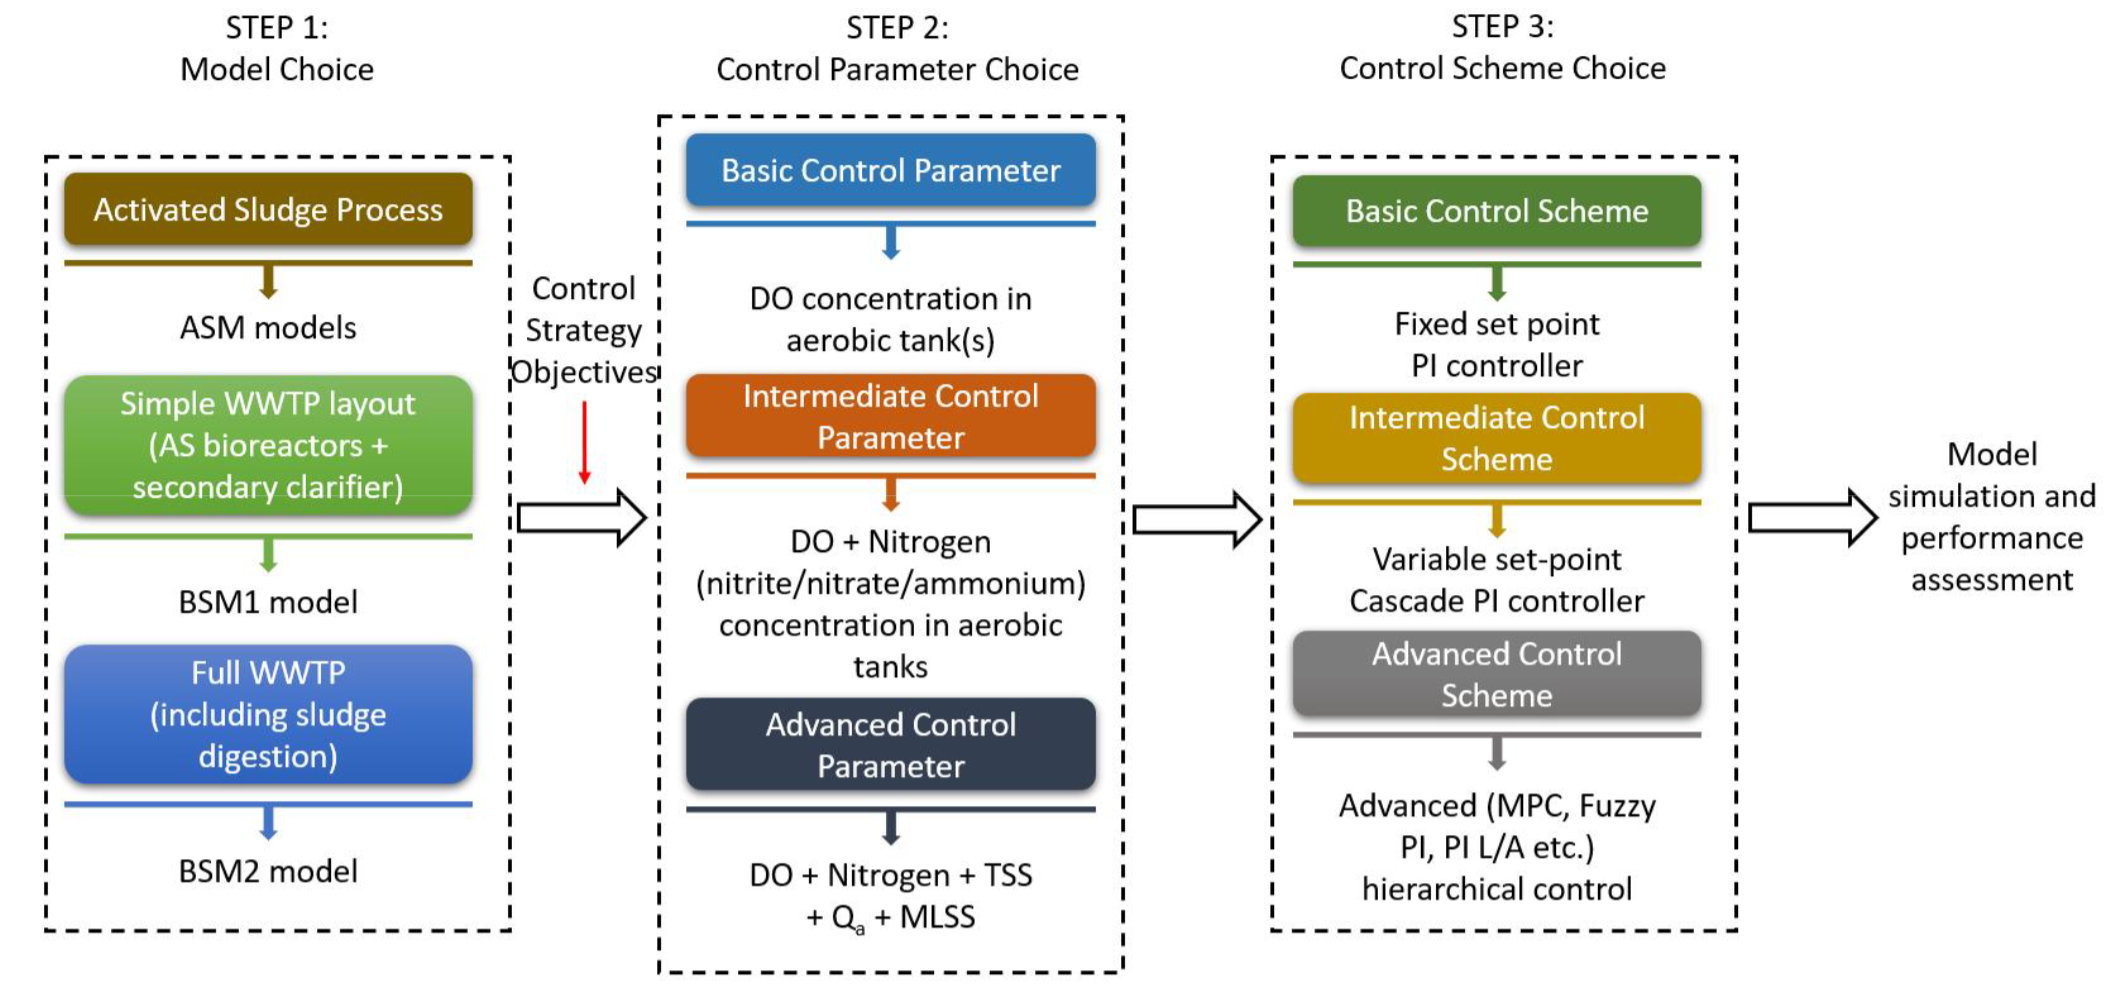
\includegraphics[width=0.9\columnwidth]{imgs/propose-frameworks-for-control-strategy-design.png}
   \caption{Proposed framework for control strategy design by \citet{ballhysaWastewaterTreatmentPlant2020}.}
   \label{fig:control-strategy-design}
\end{figure}
 
In recent years, many publications presented an exciting way to demonstrate how machine learning-based model predictive control (MPC) can outperform the conventional PID controller in WWTPs using BSM. The researchers use Matlab-Simulink to simulate the treatment processes in WWTPs. At the same time, the block of PID controllers is replaced with machine learning models, and the effluent quality or treatment system performance can be differentiated via BSM simulated results. \citet{wangModelPredictiveControl2020} compared the stability of chlorinated water quality in the effluent of a DWTP with two control strategies, which are PID feedback controls and a predictive model-based support vector machine (SVM). The BSM simulated results showed that the SVM model required 21 minutes less to reach the residual chlorine setpoint than PID feedback controls. A proposed neuro-fuzzy PID controller (i.e., a hybrid machine learning model consisting of neural networks and fuzzy logic) also showed superior performance in optimizing the chlorine dosing rate to minimize the chance of errors \citep{hongApplicationNeurofuzzyPID2012}. The significance of using BSM in Matlab-Simulink enables the performance of traditional and machine learning-based control strategies can be compared in objective and fair senarios, also providing the practicability of machine learning to the experts in the field. Matlab is a powerful and resourceful platform providing various machine learning functions, including point-and-click apps for training and evaluation, available classification and regression algorithms, Automatic machine learning (AutoML), etc \citep{mathworksMATLABMachineLearning2022}. The direct access to the abundant features and the integration of Simulink make Matlab an appealing option for many researchers in the wastewater treatment industry, especially in the research domain of machine learning and control strategy simulation. Despite the countless benefits of using Matlab, the Python programming language stands out differently.

Python is a high-level, interpreted, and object-oriented programming language and features simple and easy-to-learn syntax providing good readability \citep{WhatPythonExecutive}. The large developer community (e.g., GitHub and Stackoverflow) and open-source access (i.e., free of charge) have made Python an ideal tool for machine learning starters. The most cutting-edge research in the field of Artificial Intelligence is often led by Tech Giants like Google and Amazon, which conduct research via Python (e.g., machine learning frameworks of TensorFlow (Google)in Python), as well as the big research community using Python. All the latest updates and developments relating to machine learning architectures and techniques are usually accessible in the open-source Python community, including the example codes. Contrary to Python, users of commercial software Matlab need to wait for the software engineers working in Matlab to update the latest machine learning applications onto the Matlab platform, which is a time-consuming process and creates a delay of time and accessibilities to many resources \citep{castroWhyShouldChoose2018}. Machine learning developers in the wastewater treatment industry can freely choose between the programming methods based on the research need. Those looking for mature machine learning algorithms can simply use Matlab and be satisfied with the functionalities; on the other hand, those who intend to incorporate more new techniques and architectures in machine learning models can consider using Python as the programming language. Interestingly, MathWorks recently announced using Python functions in Simulink Model \citep{mathworksCallPythonFunction2022}; despite the update from Matlab, to the best of my knowledge, there are no research papers developing machine learning algorithms on Python and running on Matlab-Simulink. 

\subsection{Data pre-processing}
The ubiquitous sensors installed in WWTPs for treatment automation generate a massive amount of data on a daily basis. Before being used for any purposes, the data must be understandable for explanation and relevant enough for water experts to extract valuable information \citep{kehreinCriticalReviewResource2020}. Without the help of Artificial Intelligence, data manipulation before training machine learning models can be time-consuming and challenging. The specifically designed algorithms can perform data evaluation and augmentation to improve data quality. Any statistical or machine learning algorithms which can complete these tasks are known as the data pre-processing techniques. The causes of sensors rendering undesired data with low quality are the limitations of the hardware sensors and the dynamics of the sampling locations. In general, the false data generated by sensors can be described in eight distinct states \citep{rosenAddingRealismSimulated2008,newhartDatadrivenPerformanceAnalyses2019}:

\noindent
\begin{myenumerate}
    \item Operational: Sensor is working properly with normal measurement noise.
    \item Excessive drift: When a sensor outputs a value progressively further from the truevalue.
    \item Shift: When the output of the sensor is a constant amount away from its true value.
    \item Fixed value: When the sensor is stuck and keeps repeating the same value.
    \item Complete failure: Similar to a fixed value fault, but the sensors either give offthemaximum or minimum, value, zero or no value at all.
    \item Wrong gain: When signals away from the calibration point are under- orover-amplified bythe sensor.
    \item Calibration: The sharp change in sensor output directly following a calibration.
    \item Isolated fault: When a single point in a series shows an incorrect value.
\end{myenumerate}

The researchers and experts have been proposing solutions for filling the data gaps created by sensor faults and maintenance operations. However, the number and length of missing values are mainly subject to the dynamics of the system being monitored and other factors. In their open-source wastewater data treatment toolkit,\citet{demulderOpenSoftwarePackage2018} has recommended five data imputation strategies aimed at data generated from water resource recovery facilities:

\noindent
\begin{myenumerate}
    \item Interpolate.
    \item Use a correlation with other available measurement signals.
    \item Replace with a corresponding value in an average daily profile.
    \item Repeat the values obtained on the preceding day.
    \item Replace with the output of a model. 
\end{myenumerate}

The efficient monitoring of sensors and proper use of the data for developing control strategies in the wastewater treatment industry rely on careful data quality control. In recent years, automated data evaluation has drawn the attention of experts and researchers in this field as manual detection of sensor fouling is unrealistic because the tasks are labor-intensive and laborious. \citet{alferesValidatingDataQuality2013} presented three practical approaches for data quality validation, which are capable of automated calculating single abnormal values and collective faults over a long period. The author claimed that the significance of the research work is performing a data quality validation scheme on the multivariate dataset. The pitfall of the study is that despite the promising approaches proposed, the validity still depends on the thresholds or acceptability limits in the actual WWTPs. Similar to the data imputation strategies, the real situation differs tremendously across different WWTPs. That being said, instead of providing general guidance on how to manipulate data, the focus should be emphasized on how to use algorithms to help users understand, analyze, and process the fouling data.

\subsection{Feature engineering}
Feature engineering aims to enrich the raw dataset by selecting, manipulating, and transforming data, which forms a better dataset relating to the underlying targets to be learned by the machine learning model. Feature engineering and data pre-processing are easily confused with each other. The fundamental difference between the two is that the former creates essential features not included in the raw data; the latter is a data noise removal and cleaning process. In the study of \citet{mamandipoorMonitoringDetectingFaults2020}, feature engineering was performed to generate five extra features, which are the statistical metrics of mean, maximum, minimum, variance, and standard deviation of a specific input feature. However, in comparing the final results, the author only emphasized evaluating model accuracies across varied machine learning models (i.e, PCA-SVM and LSTM models). Another interesting technique used by \citet{zaghloulDevelopmentEnsembleMachine2021} is to create the gradient values of an input variable to assist the model in better learning the trend of the historical removal rate of water parameters in aerobic granular sludge reactors. Similar to the results shown in the work of \citet{mamandipoorMonitoringDetectingFaults2020}, the influence of how engineered features affect the ultimate model accuracy is excluded in the results and discussion part. Thus, creating a lack of knowledge in how significant the feature engineered inputs are to the model accuracy and which techniques can be used in which senarios. 

There is considerable ambiguity concerning the necessity of using feature-engineered inputs in training predictive models in WWTPs. In predicting total nitrogen (TN) in the effluent, \citet{guoPredictionEffluentConcentration2015} input nine features and performed feature sensitivity analysis, which can capture the change of the output values attributed to the change input. The result showed that the top three most significant inputs, temperature, TN flow, and pH, are critical in predicting TN. The author claimed physical related cause-and-effect relationships between the effluent TN and those top three effective features could be elucidated by the machine learning model. In another work on predicting influent BOD concentration, the study clearly stated that using five inputs instead of three will cause model overfitting. Three inputs for model training were considered sufficient \citep{alsulailiArtificialNeuralNetwork2021}. Variables created from feature engineering have no physical properties, leading to extra unexplainable essence in addition to the black-box nature of machine learning models. Besides, extra model inputs from feature engineering can also cause overfitting if the data quality is not carefully evaluated. Said by Andrew Ng, "Coming up with features is difficult, time-consuming, requires expert knowledge. Applied machine learning is basically feature engineering". From the quote and the recent studies, we are uncertain how feature engineering techniques can practically help the development of machine learning models in the wastewater treatment industry. More research is required to elucidate further the effectiveness of performing feature engineering.